\chapter{用于喷注标记的ParticleNet深度神经网络}
\label{chap4}
\fontsize{12bp}{14.4pt}

喷注是是LHC(大型强子对撞机)上无处不在且蕴含大量粒子信息的物理对象,因此,关于喷注的标记就是许多潜在新物理的探寻与标准模型测量检验的关键,而喷注标记任务主要分为以下三类:
\begin{enumerate}
    \item 重夸克喷注标记
    \item 重共振态标记
    \item 夸克/胶子的区分鉴别
\end{enumerate}

而分类标记任务,也是机器学习领域最活跃的方向之一。因此,要结合以上两个领域,关键性的问题就是:\textbf{怎样尽可能物理地把喷注表示成机器学习中的对象?}
\section{喷注表示方式}
从深度学习的计算机视觉领域出发,最经典的方式是表示成图像,如\ref{dl:image}所介绍。还有一种路径是把喷注表示成粒子的集合,如\ref{dl:particle}所介绍。这两种路径的表示方法在CMS实验分析中已经有了相关的探索和标记器的开发。但我们还应该保持好奇:是否还有更好的表示方法和与之对应更好的网络架构呢?

这就是我们开发的标记器所采用的喷注表示方法的基础:点云(Paticle Clouds)。点云,就是空间中数据点的集合,这类数据结构的收集方式是通过三维扫描测量物体表面周围的大量点而得到。但对于我们关心的物理喷注,应当不仅仅用点云,或者说,应该用点云的一个喷注适应版:粒子云\cite{PaticleNet}(Particle Cloud)。

喷注(或者说,粒子云)就是空间中粒子的集合。粒子云的收集方式是用粒子探测器测量到的大量粒子的聚类。

经过喷注适应后的粒子云表示方式和点云表示方式有如下的关联:
\begin{itemize}
    \item 共同点:点云中的点和粒子云中的粒子都是内禀无序的。
    \item 不同点:点云中的基本信息是xyz空间的3维坐标;粒子云中的基本信息是$\eta-\phi$空间的二维坐标,但同时还具有许多其他特征,如:能动量,电荷,粒子鉴别(Particle ID),径迹质量,探测器受击参数等。
\end{itemize}
粒子云的置换对称性使其成为喷注最自然和有希望的表示。为了实现粒子云表示的最佳性能,必须仔细设计神经网络的架构以充分利用这种表示的潜力。在本节中,我们将介绍ParticleNet,这是一种类似于CNN的深度神经网络,使用粒子云数据进行喷注标记。
\section{边卷积(EdgeConv)}
CNN在计算机视觉的各种机器学习任务中取得了压倒性的成功。CNN的两个关键特征对其成功做出了重大贡献。首先,卷积操作通过在整个图像中使用共同核函数来利用图像的平移对称性。这不仅大大减少了网络中的参数数量,而且可以更有效地学习参数,因为每个卷积矩阵都会使用图像的所有位置进行学习。其次,CNN利用分层方法学习图像特征。卷积操作可以有效堆叠形成深度网络。CNN中的不同层具有不同的感知范围,因此可以学习不同尺度的特征,浅层利用局部定域信息,深层学习更多全局结构。这种分层方法被证明是了一种学习图像的有效方法。

受到CNN的启发,ParicleNet中采用了类似的方法来学习粒子云数据。然而,常规的卷积运算不能应用于粒子云,因为粒子云中的点可以不规则不均匀地分布,而不是像图像中的像素一样被划分为均匀的网格。因此对于粒子云结构,其卷积操作的基础,即卷积核函数如何作用于不均匀不规整的局域数据点,仍然有待定义。此外,一个通常的卷积操作,是这样的形式$\sum_{i}K_{i}x_{i}$,这里$x_i$
表示局域某个点的特征,$K_i$是核函数对应该点的矩阵元。我们可以看到,这个形式在点的置换操作下是会变的(交换$x_i$,$x_j$而不交换$K_i$,$k_j$)。因此,适应于粒子云的“卷积”操作也需要修改以考虑到粒子云内的交换对称性。

边卷积(EdgeConv)操作\cite{edgeconv}被提出作为点云结构的类卷积操作。EdgeConv 首先将点云表示为图结构,其顶点(Vertex)是点本身,为每个点与其k个最近的相邻点的连线被构造为图的边(Edge)。这样,为每个点定义了点云卷积所需的局部补丁作为与之相连的最近邻点。每个点的EdgeConv操作有形式
\begin{equation}\label{eq:4.1}
    \bm{x}_{i}^{\prime}=\mathop{\square}\limits_{j=1}^{k}\bm{h}_{\bm{\Theta}}(\bm{x}_{i},\bm{x}_{i_{j}}),
\end{equation}
这里$\bm{x}_{i}\in\mathbb{R}^{F}$表示点$x_i$的特征向量,$\{i_{1},...,i_{k}\}$是点$x_i$的k最近邻点的索引,边函数$\bm{h}_{\bm{\Theta}}:\mathbb{R}^{F}\times\mathbb{R}^{F}\rightarrow\mathbb{R}^{F^{\prime}}$代表着一系列可被$\bm{\Theta}$参数化的函数,且$\bm{\Theta}$本身属于可学习参数。$\square$是逐通道的对称聚合操作(例如max,mean,sum等)。并且边函数$\bm{h_\Theta}$对于点云中的所有点都是相同的,这样和对称聚合操作$\square$一起使边卷积(EdgeConv)成为了点云上的置换对称操作。

在ParticleNet模型中,遵循了以上原则,并且使用了特殊化的边函数
\begin{equation}
    \displaystyle\bm{h}_{\bm{\Theta}}(\bm{x}_{i},\bm{x}_{i_{j}})=\displaystyle{Conv}_{\bm{\Theta}}(\bm{x}_{i},\bm{x}_{i_{j}}-\bm{x}_{i})=\displaystyle\sum_{c}\theta_{c}^{~{}a}x_{i,c}+\sum_{c}{\theta^{\prime}}_{c}^{~{}a}(x_{i_{j},c}-x_{i,c})
\end{equation}
在这里,方程\eqref{eq:4.1}中的邻点的特征向量$\bm{x}_{i_{j}}$被$\bm{x}_{i_{j}}$与中心点的特征向量$\bm{x}_{i}$的差值所取代,并且$Conv_{\bm{\Theta}}$仅是常规形式下特征向量的加权和。c是输入特征向量序列的索引,a是核函数序列的索引。对于方程\eqref{eq:4.1}中的对称聚合操作$\square$,ParticleNet采取的是平均值$\frac{1}{k}\sum$。

\begin{figure}[H]
 \centering
 \caption{边卷积(EdgeConv)操作的结构\cite{PaticleNet}}
 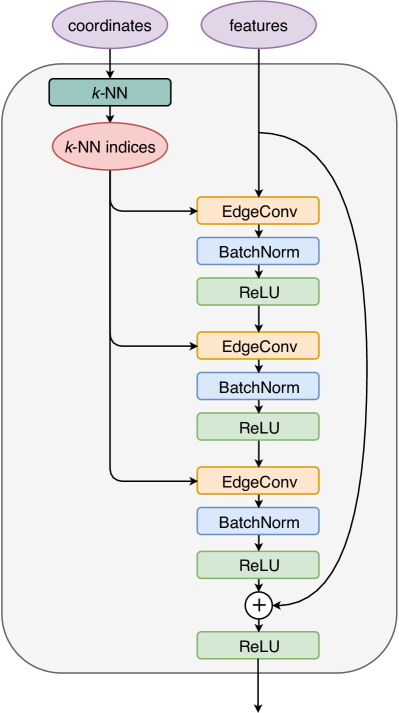
\includegraphics[height=14cm, width=8cm]{pictures/edgeconv.png}
 \label{fig:4.1}
\end{figure}

EdgeConv 操作的一个重要特点是它可以很容易地堆叠,就像常规卷积一样。这是因为 EdgeConv可以看作是从一个点云到另一个具有相同数目点的点云的映射,只是可能会改变每个点的特征向量的维度。因此,随后可以应用另一个 EdgeConv 操作。这使我们能够使用EdgeConv操作构建一个深度网络,该操作可以分层学习点云的特征。

EdgeConv 操作的可堆叠性也带来了另一个有趣的可能性。基本上,EdgeConv 学习到的特征向量可以看作是潜在空间中原始点的新坐标,然后是点之间的距离(用于判断最近的邻居)可以在这个潜在空间中重新定义。换句话说,点的接近程度可以动态地通过EdgeConv操作学习到。这也是了动态图卷积神经网络的结果Wang(2018)。其中描述点云的图被动态更新以反映边的变化,即每个点的邻居,这也得到证明比保持静态图 的性能更好。Wang等人(2018) .

\section{ParticleNet网络架构}
ParticleNet架构大量使用了EdgeConv操作,也采用了动态图更新方法。然而,与原始的Dynamic Graph CNN相比,ParticleNet中做出了许多不同的设计选择,以更好地适应喷注标记任务。

\begin{figure}[H]
 \centering
 \caption{ParticleNet深度网络架构\cite{PaticleNet}}
 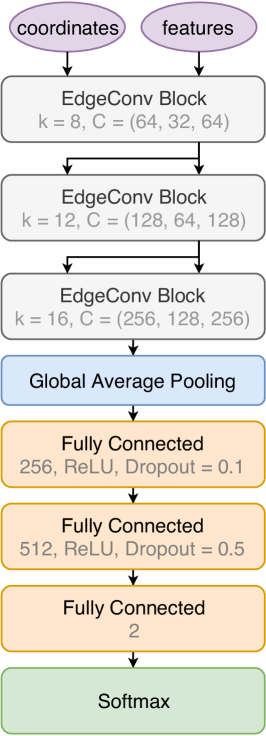
\includegraphics[height=14cm, width=5cm]{pictures/ParticleNet_Architecture.png}
 \label{fig:4.2}
\end{figure}

我们在 EdgeConv 操作块中构建 ParticleNet 架构。图1说明了 EdgeConv 块的结构。EdgeConv 块从找到每个粒子的最近相邻粒子。使用 EdgeConv 块的坐标输入计算粒子之间的距离。然后,对粒子的输入特征向量应用 EdgeConv 操作。每个块由多个 EdgeConv 操作组成,可能具有不同数量的卷积核。在每个块内,描述粒子云的图是固定的,即一个粒子总是有相同的最近的邻居。每个 EdgeConv 操作后面都有一个批量归一化层BatchNorm【Ioffe 和 Szegedy (2015)】然后是 ReLU 非线性Glorot 等人。(2011) . 与 ResNet 类似,与 EdgeConv 操作并行运行的快捷连接也包含在每个块中。


本文使用的 ParticleNet 架构如\textbf{图\ref{fig:4.2}}所示。它由三个 EdgeConv 块组成。第一个EdgeConv块使用伪快速度-方位角空间中粒子的空间坐标来计算距离,而随后的块使用学习的特征向量作为坐标。最近邻居的数量对于三个块,分别为 8、12 和 16。每个块由三个 EdgeConv 层组成。三个块的 EdgeConv 层的输出通道数为 (64, 32, 64), (128, 64, 128) 和 (256, 128, 256)。在 EdgeConv 块之后,应用全局平均池化操作来聚合云中所有粒子的学习特征。接下来是两个全连接层,分别有 256 和 512 个单元。两者都使用 ReLU 激活函数。两个带有dropout概率分别为0.1和0.5的dropout层用来以防止过度拟合。然后是具有2个单元的全连接层,后跟一个softmax函数,用于生成二分类任务的输出。

